\documentclass[runningheads,deutsch]{llncs}
%
\usepackage[T1]{fontenc}
%
\usepackage{graphicx}
%

% Daniel Motz's packages
\usepackage{etoolbox}
\makeatletter
\let\llncs@addcontentsline\addcontentsline
\patchcmd{\maketitle}{\addcontentsline}{\llncs@addcontentsline}{}{}
\patchcmd{\maketitle}{\addcontentsline}{\llncs@addcontentsline}{}{}
\patchcmd{\maketitle}{\addcontentsline}{\llncs@addcontentsline}{}{}
\setcounter{tocdepth}{3}
\makeatother
\usepackage{bookmark}

\usepackage{amsfonts}
\usepackage{amsmath}
\usepackage{stmaryrd}
\usepackage{amssymb}
\usepackage{mathtools}
\usepackage{ bbold }
\DeclarePairedDelimiter\ceil{\lceil}{\rceil}
\DeclarePairedDelimiter\floor{\lfloor}{\rfloor}

\usepackage{tikz}
\usepackage{pgfplots}
\pgfplotsset{compat = newest}
\usetikzlibrary{arrows, automata, positioning}

\usepackage{hyperref}

\usepackage{setspace}
\doublespacing

\renewcommand{\abstractname}{}
\newcommand{\inline}{\mintinline[fontsize=\normalsize]{c++}{text}}
\DeclareUnicodeCharacter{03BB}{$\lambda$}
% END Daniel Motz's packages

\begin{document}
%
\title{
    Automaten und Berechenbarkeit \\
    Dr. Jörg Vogel \\
    Skript zur VL im WS 2021
}
%
\titlerunning{
    Automaten \& Berechenbarkeit
}%
\author{
    Dr. Jörg Vogel \and 
    Maximilian Stock \and 
    Daniel Motz
}
%
\authorrunning{Vogel, Stock, Motz}
%
\institute{Fakultät für Mathematik und Informatik, Friedrich-Schiller-University,\\ Jena, Germany\\
\vspace{.2cm}
\email{\{maximilian.stock, daniel.motz\}@uni-jena.de}
}
%
\maketitle
%
\pagebreak

\section{Endliche Automaten und reguläre Sprachen}

\subsection{Alphabete, Wörter und Sprachen}

Die Darstellung von Daten -- als Eingabe für Algorithmen -- wird realisiert als "Wörter".

\begin{example}
    Darstellung von Graphen

    \begin{minipage}{.5\textwidth}
        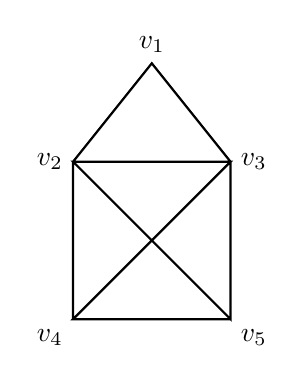
\begin{tikzpicture}[domain=0:4]
            \draw[thick,sharp corners=0pt]
            (0,0) node[anchor=north east]{$v_4$} --
            (0,2) node[anchor=east]{$v_2$} -- 
            (1,3.25) node[anchor=south]{$v_1$} --
            (2,2) node[anchor=west]{$v_3$} -- 
            (2,0) node[anchor=north west]{$v_5$} -- 
            (0,2) --
            (2,2) -- 
            (0,0) -- 
            (2,0);
        \end{tikzpicture}
    \end{minipage} %
    \begin{minipage}{.5\textwidth}
        $\begin{matrix}
            & v_1 & v_2 & v_3 & v_4 & v_5 \\
        v_1 & 0 & 1 & 1 & 0 & 0 \\
        v_2 & 1 & 0 & 1 & 1 & 1 \\
        v_3 & 1 & 1 & 0 & 1 & 1 \\
        v_4 & 0 & 1 & 1 & 0 & 1 \\
        v_5 & 0 & 1 & 1 & 1 & 0
        \end{matrix}$
    \end{minipage}%
    \newline%
    \newline%
    Codewort: $\#0100\#10111\#11011\#01101\#01110\#$
    $\rightarrow$ Buchstaben aus $\{0, 1, \#\}$
\end{example}

\begin{definition}
    Ein Alphabet $\Sigma$ ist eine endliche nicht leere Menge.
\end{definition}

\begin{example}
    \begin{align}
        \Sigma_{\text{graph}} &= \{ 0, 1, \# \} \\
        \Sigma_{\text{latein}} &= \{ a, b, c, \dots, x, y, z \} \\
        \Sigma_{\text{griech}} &= \{ \alpha, \beta, \gamma, \dots, \omega \} \\
        \Sigma_{\text{boole}} &= \{0, 1\} = \Sigma_{bin} \\
        \Sigma_{\text{dezi}} &= \{0, 1, \dots, 9\} \\
        \Sigma_{\text{unär}} &= \{1\} \\
        \Sigma_{\text{Tastatur}} &= \{a, b, c, \dots, z\} \cup \{A, B, C, \dots, Z\} \cup \{\text{ä}, \text{Ä}, \dots\} \\
        &\phantom{==} \cup \{0, \dots, 9\} \cup \{!, \backslash, \#, ;, -, ~, \dots\} \cup \{\text{␣}\}
    \end{align}
    $\hookrightarrow \emptyset, \mathbb{N}$ sind keine Alphabete
\end{example}

\begin{definition}
    Es sei $\Sigma = \{a_1, a_2, \dots, a_m\}$ ein Alphabet mit $m$ Buchstaben. Ein Wort $w$ ist eine endliche Folge von Buchstaben aus $\Sigma$, etwa:
    \[ w = a_{i1} \; a_{i2} \; \dots \; a_{in}, \quad a_{ij} \in \Sigma \]
    Die Länge dieses Wortes ist $n$ -- die Anzahl seiner Buchstaben.
    \begin{note}
        $|w| = n$
    \end{note}
    Sonderfall: Das leere Wort $\lambda$ hat die Länge 0. \\
    $\Sigma^*$ bezeichnet die Menge aller (endlichen) Wörter über $\Sigma$.

    \begin{align}
        \Sigma^0 &:= \{\lambda\} \\
        \Sigma^{n+1} &:= \Sigma^n \cdot \Sigma := \{wa\;|\;w \in \Sigma^n,\;a \in \Sigma\} \\
        \Sigma^* &:= \bigcup_{n\in \mathbb{N}} \Sigma^n
    \end{align}
\end{definition}

Für die Länge gilt: $|\lambda| = 0 \quad , \quad |wa| = |w| + 1$
\[ w \in \Sigma^n \leftrightarrow |w| = n \]

\begin{remark}
    Was sind Wörter über $\Sigma_{\text{Tastatur}}$?
    \begin{itemize}
        \renewcommand{\labelitemi}{$\rightarrow$}
        \item Wörter der natürlichen Sprache
        \item Zahlen
        \item Sätze, Texte, Romane, \dots 
        \item Graphen
    \end{itemize}
    $\hookrightarrow$ Der Begriff Wort ist in der Informatik ein anderer als in der Umgangssprache. Alle Informationen, alle Daten, ... sind Wörter.
\end{remark}

\pagebreak

\subsubsection{Operationen für Wörter}
\paragraph{Konkatenation / Hintereinanderschreiben}\phantom{ }\\
    Für zwei Wörter
    \begin{align*}
        u &= x_1\, x_2\, \dots\, x_n \\
        v &= y_1\, y_2\, \dots\, y_k
    \end{align*}
    mit $x_i, y_j \in \Sigma = \{ a_1, a_2, \dots, a_m \}$ ist
    \[ u \circ v := x_1\, x_2\, \dots\, x_n\  y_1\, y_2\, \dots\, y_k \]
    die Konkatenation von $u$ und $v$.\\
    
    Es ist damit eine zweistellige assoziative Operation: $(u\circ v)\circ w = u \circ (v\circ w)$ mit der Eigenschaft $u\circ \lambda = u = \lambda \circ u$. Das heißt $\lambda$ ist das neutrale Element.

    Die Struktur $(\Sigma^*, \circ, \lambda)$ ist ein Monoid und heißt \textit{freie Worthalbgruppe} über $\Sigma$. (Auch $(\mathbb{N}, \circ, \lambda)$ ist ein Monoid.)

    % TODO wieso heißt die Abbildung |\cdot|?
    Die Abbildung $|\cdot|: \Sigma^* \mapsto \mathbb{N}$, die jedem Wort seine Länge zuordnet, ist ein Homomorphismus von $\Sigma^*$ auf $\mathbb{N}$, denn es gilt: $|u \circ v| = |u| + |v|$.

\begin{note}
    $w = u\circ v$ immer, wenn "algebraisch". \\
    aber praktisch: ohne $\circ$, sondern $w = uv$.
\end{note}

\subsubsection{Potenzen von Wörtern}
Es sei $w = x_1\, x_2 \, \dots \, x_n \in \Sigma^*$ ein (beliebiges) Wort der Länge $n$. Wir definieren (rekursiv):

\begin{align}
    w^0 &:= \lambda \\
    w^1 &:= w \\
    w^k+1 &:= w^k \circ w
\end{align}

Die \textit{k-te Potenz} eines Wortes $w$ ist das Wort $w$ k-mal konkateniert.

\begin{example}
    $w = baa\, baa\, abab$ über $\Sigma = \{a, b\}$
    \begin{align*}
        w &= (baa)^2 \, (ab)^2 \\
        &= b^1\, a^2 \, b^1\, a^3\, b^1\, a^1\, b^1
    \end{align*}
\end{example}

Damit haben wir folgende Schreibweise: für $\Sigma = \{a\}$:
\[ \Sigma^* = \{\lambda, a, a^2, a^3, ..., a^n, \dots \} \]

\subsubsection{Spiegelwort}

Für ein Wort $w = x_1\, x_2\, x_3\, \dots \, x_{n-1}\, x_n \quad (x_i \in \Sigma)$ ist das Spiegelwort
\[ \text{Sp}(w) := x_n\, x_{n-1}\, \dots \, x_3\, x_2\, x_1 := w^R \]
\text{Sp} ist eine einstellige Operation, für die gilt:
\begin{align}
    \text{Sp}(\lambda) &= \lambda \\
    \text{Sp}(a) &= a \quad (a \in \Sigma) \\
    \text{Sp}(wa) &= a \text{Sp}(w) \quad (a \in \Sigma, w \in \Sigma^*)
\end{align}

\subsection{Relationen für Wörter}

\begin{definition}
    Es seien $u, w \in \Sigma^*$. $u$ ist ein Teilwort von $w \xleftrightarrow[\text{def.}]{}$ es gibt zwei Wörter $l, r \in \Sigma^*$, sodass $w=lur$.
\end{definition}


\begin{note}
    $u$ ist Teilwort von $w$: $u \sqsubseteq w$
\end{note}

\begin{example}
    $\Sigma := \{a, b\}, \quad w = ab\, ab\, ab\, ba\, bb, \quad |w| = 10$

    Alle Teilwörter der Länge 4: $abab, baba, \textcolor{gray}{abab}, babb, abba, bbab, \textcolor{gray}{babb}$
\end{example}

\begin{remark}
    $l = \lambda$ oder $r = \lambda$ ist zugelassen. Falls $l = \lambda$, dann gilt: $w = ur$. In diesem Fall heißt $u$ \textit{Präfix (Anfangswert)} von $w$.

    Falls $r = \lambda$, dann gilt: $w = lu$. In diesem Fall heißt $u$ \textit{Suffix (Endwert)} von $w$.
\end{remark}

\begin{remark}
    Jedes Teilwort ist eine zusammenhängende Folge von Buchstaben von $w$
\end{remark}

\begin{property}
    Eigenschaften von $\sqsubseteq$

    Es gilt: $\sqsubseteq\, \subseteq \Sigma^* \times \Sigma^*$ mit
    \begin{itemize}
        \item Reflexivität
        \item Transitivität
        \item Antisymmetrie
    \end{itemize}
    Damit ist $\sqsubseteq$ eine Halbordnungsrelation über $\Sigma^*$, wobei $\lambda \sqsubseteq w$ für alle $w \in \Sigma^*$.
    Damit ist $(\Sigma^*, \sqsubseteq, \lambda)$ eine halbgeordnete Menge mit dem Minimum $\lambda$.
    \color{gray} Wir wissen $(\mathbb{N}, \leq, 0)$ ist eine halbgeordnete Menge mit dem Minimum 0.
    Analogie: $(\Sigma^*, \circ, \lambda)$ und $(\mathbb{N}, + 0)$ sind Monoide mit dem Homomorphismus $u \circ v = |u| + |v|$ von $\Sigma^*$ auf $\mathbb{N}$.
    \color{black}
\end{property}

\subsubsection{Binäre Nummern und Binärdarstellung}
Es ist $\Sigma_{\text{bin}} = \{0, 1\}$. Weiter sei $w = x_1\, x_2\, \dots\, x_n \in \Sigma^*_{\text{bin}}$ für $n > 0$. \textcolor{gray}{$w \neq \lambda$}

Die \textit{binäre Nummer} von $w$ ist definiert als

\[ \text{Nr}_\text{bin}(w) := \Sigma^n_{i=1} x_i \cdot 2^{n-1} \]

Die \textit{Binärdarstellung} von $n$ ist das kürzeste Wort $w \in \{0, 1\}^*$ mit $\text{Nr}_\text{bin}(w) = n$.

\begin{example}
    Es sei $w = 00\, 11\, 01\, 10$ mit $|w| = 8$. Also ist 
    \begin{align*}
        \text{Nr}_\text{bin}(w) &= \Sigma^8_{i=1} x_i \cdot 2^{8-i} \\
        &= 0 \cdot 2^7 + 0 \cdot 2^6 + 1 \cdot 2^5 + 1 \cdot 2^4 + 0 \cdot 2^3 + 1 \cdot 2^2 + 1 \cdot 2^1 + 0 \cdot 2^0
        &= 54
    \end{align*}

    Andererseits ist $\text{bin}(54) = 11\, 01\, 10$
\end{example}

Wir wissen: Binärdarstellungen sind solche Wörter $w\in \{ 0,1 \}^* \backslash \{\lambda\}$, die mit $1$ beginnen oder $w=0$. Für jede natürliche Zahl $n$ gibt es unendliche viele Wörter $w$ mit $\text{Nr}_{\text{bin}}(w) = n$. Das ist das "Gegenteil" von eineindeutiger Zuordnung!

\subsubsection{Kanonische Ordnung und dyadische Darstellung}

Es sei $\Sigma = \{ a_1, a_2, \dots, a_m \}$ ein beliebiges Alphabet mit der natürlichen Ordnung $a_1 < a_2 < \dots < a_m$. Zum Beispiel $\Sigma_{\text{latein}} = \{a < b < c \dots < x < y < z\}$ und $\Sigma_{\text{dezi}} = \{0 < 1 < 2 \dots < 9\}$

Frage: Warum lässt sich die übliche natürliche Ordnung (wie im Duden) nicht für $\Sigma^*$ nicht benutzen?

$\rotatebox[origin=c]{180}{$\Lsh$}$ Im Duden stehen endlich viele Wörter, $\Sigma^*$ umfasst unendlich viele Wörter! Zählt man die Wörter aus $\Sigma^*$ in der natürlichen Ordnung auf, ergibt sich $a_1, a_1, a_1, a_1, a_1, a_1, \dots \rightarrow$ auf diese Weise wird $a_2$ gar nicht erreicht!

\begin{definition}
    Es seien $u, v \in \Sigma^*$. Die kanonische Ordnung (quasilexikographische Ordnung) (Schreibweise: $u < v$) ist definiert durch
    \begin{enumerate}
        \item $|u| < |v|$
        \item Wenn $|u| = |v|$ und es gibt einen Präfix $p$, sodass gilt: $u = p\, a_i\, u_R$ und $v = p\, a_j\, v_R$ und $a_i < a_j$ in der natürlichen kananonischen Ordnung??
        % TODO herausfinden was nicht mehr auf dem Scan zu sehen ist.
    \end{enumerate}
\end{definition}

\begin{example}
    $\Sigma_{\text{bin}} = \{0,1\}$ mit $0 < 1$.

    $\Sigma^*_{\text{bin}} = \{ \lambda, 0, 1, 00, 01, 10, 11, 000, 001, \dots \}$ ist die kanonische Ordnung für $\{0, 1\}^*$.
\end{example}

Wir betrachten jetzt das Alphabet $\Sigma^*_{\text{dya}} = \{1, 2\}$ mit $1 < 2$.
Die kanonische Ordnung für $\{1, 2\}^*$ ist 

\[ \Sigma^*_{dya} = \{ \lambda,1, 2, 11, 12, 21, 22, 111, 112, \dots \} \]

mit den Platznummern $0, 1, 2, 3, 4, 5, 6, 7, 8, \dots$

für die gilt: $1\cdot 2^0,\ 2\cdot 2^0,\ 1\cdot 2^1 + 1\cdot 2^0,\ 1\cdot 2^1 + 2\cdot 2^0, \dots$

Für $\Sigma_{dya}$ und ein $w\in \Sigma_{dya}^* = \{1, 2\}^*$ mit $w = x_1\, x_2\, \dots, x_n (w \neq \lambda)$
definieren wir

\[ \text{Platznummer}(w) = \sum^n_{i=1} x_i \cdot 2^{n-i}, \quad \text{für}\, x_i \in \{1, 2\} \]

\textit{Fakt}: Jede positive natürliche Zahl $k$ besitzt eine eindeutige Darstellung der Form
\[ (\star)\quad k = \sum^n_{i=1} x_i \cdot 2^{n-i}, \quad \text{für}\, x_i \in \{1,2\} \]

Für eine positive natürliche Zahl mit $(\star)$ ist
\[ k = (x_1\, x_2\, \dots\, x_n)_2\]

\textit{die dyadische Darstellung von} $k$.

Wir setzen für $k=0$: $0=(\lambda)_2$. Damit haben wir:

\begin{align}
    \textit{Platznummer:}\; & \{1, 2\}^* \mapsto \mathbb{N}\; \text{und} \\
    \textit{dyadische Darstellung dya:}\; & \mathbb{N} \mapsto \{1, 2\}^*
\end{align}

wobei \textit{dya} die Umkehrabbildung von Platznummer ist. Damit ist \textit{dya} eine Bijektion zwischen $\mathbb{N}$ und $\{1,2\}^*$.

% TODO ergänzen

\section{Endliche Automaten}

\begin{example} (wenn auch ein nicht-formales): Ein Aufzug mit zwei Stockwerken
    \textbf{Mögliche Eingaben}
    \begin{enumerate}
        \item im Aufzug möchte jemand nach oben
        \item oben wartet jemand 
        \item im Aufzug möchte jemand nach unten
        \item unten wartet jemand
    \end{enumerate}

    Wir unterscheiden zwei Zustände:
    \begin{align*}
        \rightarrow & \text{"oben": der Aufzug ist oben} \\
        & \text{"unten": der Aufzug ist unten}
    \end{align*}

    \begin{center}        
        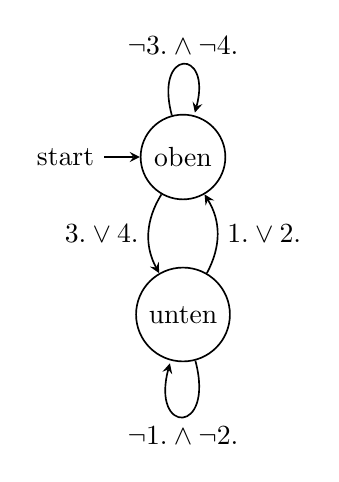
\begin{tikzpicture}[
            ->,
            >=stealth,
            semithick,
            node distance=2cm]
            \node [state,initial] (a) {oben};
            \node [state] (b) [below of = a] {unten};

            \path (a) edge [bend right,left] node {$3. \lor 4.$} (b)
                      edge [loop above,above] node {$\lnot 3. \land \lnot 4.$} (a)
                  (b) edge [bend right,right] node {$1. \lor 2.$} (a)
                      edge [loop below,below] node {$\lnot 1. \land \lnot 2.$} (b);
            
        \end{tikzpicture}
    \end{center}
\end{example}

\begin{definition}
    Ein (deterministischer) endlicher Automat $A$ ist ein $5$-Tupel $A = (Q, \Sigma, \delta, q_0, F)$, wobei:
    \begin{enumerate}
        \item $Q$ ist eine endliche nicht-leere Menge: \textit{Zustandsmenge}
        \item $\Sigma$ ist eine endliche nicht-leere Menge: \textit{Eingabealphabet}
        \item $\delta$ ist eine Funktion $\delta: Q \times \Sigma \mapsto Q$ \textcolor{gray}{mit $Q\cap \Sigma = \emptyset$} und heißt \textit{Übergangsfunktion} \textcolor{gray}{(Programm)}
        \item $q_0 \in Q$ ist der \textit{Startzustand} von $A$
        \item $F \subseteq Q$ ist die Menge der \textit{Finalzustände} von $A$
    \end{enumerate}
\end{definition}

\begin{example}
    Wir wählen $\Sigma = \{0, 1\}.$ Wir legen fest: $w := 0110 \in \Sigma^*$. Wir konstruieren einen endlichen Automaten $A_1$, der dieses $w$ "erkennt". Dies stellen wir als Graphen dar, wobei die Knoten \textit{Zuständen} und die Kanten \text{Übergängen gemäß $\delta$}.
    \\
    \\
    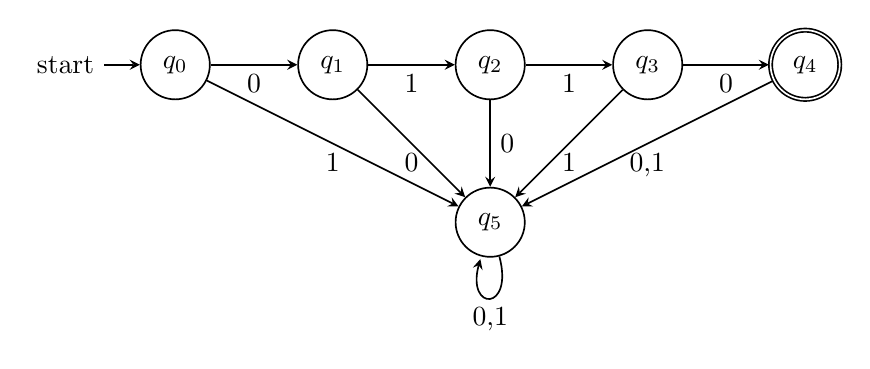
\begin{tikzpicture}[
        ->,
        >=stealth,
        semithick,
        node distance=2cm]
    
        \node [initial,state]    (0) {$q_0$};
        \node [state]            (1) [right of=0] {$q_1$};
        \node [state]            (2) [right of=1] {$q_2$};
        \node [state]            (3) [right of=2] {$q_3$};
        \node [state,accepting]  (4) [right of=3] {$q_4$};
        \node [state]            (5) [below of=2] {$q_5$};
        
        \path (0) edge [below] node {0}   (1)
                    edge [below] node {1}   (5)
                (1) edge [below] node {1}   (2)
                    edge [below] node {0}   (5)
                (2) edge [below] node {1}   (3)
                    edge [right] node {0}   (5)
                (3) edge [below] node {0}   (4)
                    edge [below] node {1}   (5)
                (4) edge [below] node {0,1} (5)
                (5) edge [loop below,below] node {0,1} (5);
    \end{tikzpicture}

    Dabei ist also:
    \begin{align*}
        Q &= \{q_0, q_1, q_2, q_3, q_4, q_5\} \\
        \Sigma &= \{0, 1\} \\
        \delta &\quad \text{gemäß des Graphen} \\
        q_0, &\quad F= \{q_4\}
    \end{align*}

    \begin{itemize}
        \item Die Überführungsfunktion $\delta$ ist total definiert.
        \item Der Automat akzeptiert ein Eingabewort $w \leftrightarrow \text{ ein Finalzustand erreicht wird}$.
        \item Unser Beispiel: die einzige Eingabe, die $A_1$ akzeptiert, ist $w = 0110$.
        \item Die von $A_1$ akzeptierte Sprache ist $L(A_1) = \{0110\}$.
    \end{itemize}
\end{example}

\begin{example}
    Dasselbe Alphabet $\Sigma = \{0,1\}$. Wir konstruieren einen endlichen Automaten $A_2$, der unendlich viele Wörter der Form $w = 0110\, u$ für $u \in \{0,1\}^*$ erkennt, also alle Wörter über $\{0,1\}$, für die $0110$ ein Präfix ist. $A_2$ ist eine \textit{Modifikation} von $A_1$ mit $L(A_2) = \{0110\,u | u\in \{0,1\}^*\}$\\
    \\

    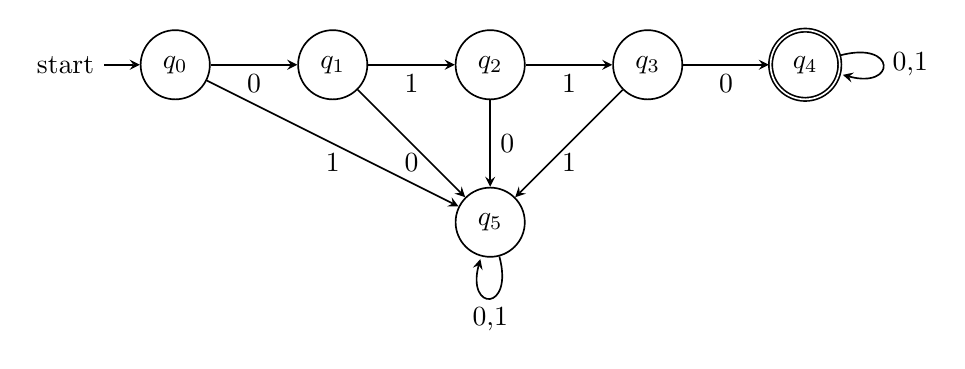
\begin{tikzpicture}[
        ->,
        >=stealth,
        semithick,
        node distance=2cm]
    
        \node [initial,state]    (0) {$q_0$};
        \node [state]            (1) [right of=0] {$q_1$};
        \node [state]            (2) [right of=1] {$q_2$};
        \node [state]            (3) [right of=2] {$q_3$};
        \node [state,accepting]  (4) [right of=3] {$q_4$};
        \node [state]            (5) [below of=2] {$q_5$};
        
        \path (0) edge [below] node {0}   (1)
                    edge [below] node {1}   (5)
                (1) edge [below] node {1}   (2)
                    edge [below] node {0}   (5)
                (2) edge [below] node {1}   (3)
                    edge [right] node {0}   (5)
                (3) edge [below] node {0}   (4)
                    edge [below] node {1}   (5)
                (4) edge [loop right, right] node {0,1} (4)
                (5) edge [loop below,below] node {0,1} (5);
    \end{tikzpicture}
\end{example}

\textit{Frage:} Wieso können $5$-Tupel eigentlich "rechnen"? $\rightarrow$ Dazu geben wir eine formale Definition der \textit{Berechnung} eines Automaten $A$ bei Eingabe $w$.

\begin{definition}
    Gegeben sei ein (deterministischer) endlicher Automat $A = (Q, \Sigma, \delta, q_0, F)$ und eine Eingabe $w\in \Sigma^*$. Eine \textit{Konfiguration $K$} von $A$ bei Eingabe $w$ ist ein Paar $K=(p, u)$, wobei $p \in Q$ (aktueller Zustand von $A$) und $u \in \Sigma^*$ (der noch zu lesende "Rest" der Eingabe $w$).

    Damit ist eine Konfiguration eine vollständige Beschreibung einer Momentsituation von $A$ bei Eingabe $w$.
\end{definition}

\begin{example}
    $A_1$ mit $0110$:

    \begin{align*}
        K_0 &= (q_0, 0110) \\
        K_1 &= (q_1, 110) \\
        K_2 &= (q_2, 10) \\
        K_3 &= (q_3, 0) \\
        K_4 &= (q_4, \lambda)
    \end{align*}
\end{example}

\begin{definition}
    Wieder sei $A = (Q, \Sigma, \delta, q_0, F)$ ein endlicher Automat und $w\in \Sigma^*$ eine Eingabe. Wir definieren eine binäre Relation $\vdash$ über der Menge der Konfigurationen: $\vdash \subseteq (Q, \Sigma^*) \times (Q, \Sigma^*)$ auf folgende Weise:
    Es gilt $K \vdash K'$ für zwei Konfigurationen $K$ und $K'$ mit $K=(p,u)$ und $K'=(q,v)$

    \[ \xleftrightarrow[\text{def.}]{} \bigvee_{x \in \Sigma} (u = xv \text{ und } \delta(p,x)=q)\]
    
    $K'$ heißt \textit{unmittelbare Nachfolgekonfiguration} von $k$. Der Übergang von $K$ zu $K'$ entspricht einem Berechnungsschritt von $A$ mit $w$ und erfolgt gemäß $\delta$. $\vdash$ heißt \textit{Übergangsrelation}.
\end{definition}

$5$-Tupel endlicher Mengen $A = (Q, \Sigma, \delta, q_0, F)$ ... \textit{ein Beispiel einer "mathematischen Maschine"} -- mit $\delta$ also "Programm", wobei $\delta$ total definiert: 

\[ \delta: Q\times \Sigma \mapsto Q \]

\textit{Konfiguration}
\[ K = (p,u) \in Q\times \Sigma^* \]

\textit{Übergangsrelation}
\[ (p,u) \vdash (q,v) \text{ taktet den Automaten} \]

Ein \textit{Takt} der Berechnung von $A$ bei Eingabe $w$ ist ein Element $((p,u), (q,v)) \in \vdash$. $(q, v)$ heißt in diesem Fall \textit{unmittelbare Nachfolgekonfiguration} von $(p,u)$.
\\
\\
\textit{Besondere Konfigurationen} \begin{itemize}%[leftmargin=1em]
    \renewcommand{\labelitemi}{$\rightarrow$}
   \item Start-Konfiguration $\text{Start-K}_A (w) := (q_0, w)$
   \item annehmende Konfiguration $\text{K}_A (w) := (q_0, \lambda) \text{ mit } q\in F$
   \item ablehnende Konfiguration $\text{K}_A (w) := (q_0, \lambda) \text{ mit } q\notin F$
\end{itemize}
Wir betrachten $\vdash^*$, die reflexive und transitive Hülle von $\vdash$.
\textit{Frage: } Wann gilt $K \vdash^* K'$? (in diesem Fall heißt $K'$ \textit{Nachfolgekonfiguration} von $K$)
\textit{Antwort:} $K \vdash^* K' \leftrightarrow \text{ es gibt eine Folge von Konfigurationen } K_0, K_1, K_2, \dots, K_t$ mit
\begin{itemize}
    \item $K_0 = K$
    \item $K_{i-1} \vdash K_i$ für $i=1, \dots, t$
    \item $K_t = K'$ (dabei ist $t$ die Taktzahl)
\end{itemize}

\end{document}
